%% uncomment to list all files in log
%\listfiles

\documentclass[12pt]{report}


\usepackage{fontspec}

%\setmainfont[Scale=MatchLowercase]{Lucida Bright}
%\setmonofont{FreeMono}
%\setmonofont{Source Code Pro}
\setmonofont[Scale=MatchLowercase]{Ubuntu Mono}

\usepackage[headings]{fullpage}

% national use characters 
%\usepackage{inputenc}

% ams mathematical symbols
\usepackage{amsmath,amssymb}

% added to support pandoc highlighting
\usepackage{microtype}

\usepackage{makeidx}

% add index and bibliographies to table of contents
\usepackage[nottoc]{tocbibind}

% postscript courier and times in place of cm fonts
%\usepackage{courier}
%\usepackage{times}

% extended coloring
\usepackage{color}
\usepackage[table,dvipsnames]{xcolor}
\usepackage{colortbl}

% advanced date formating
\usepackage{datetime}

%support pandoc code highlighting
\usepackage{fancyvrb}
\DefineShortVerb[commandchars=\\\{\}]{\|}
\DefineVerbatimEnvironment{Highlighting}{Verbatim}{commandchars=\\\{\}}
% Add ',fontsize=\small' for more characters per line

%tango style colors
% \usepackage{framed}
% \definecolor{shadecolor}{RGB}{255,255,255}
% \newenvironment{Shaded}{\begin{snugshade}}{\end{snugshade}}
% \newcommand{\KeywordTok}[1]{\textcolor[rgb]{0.13,0.29,0.53}{\textbf{{#1}}}}
% \newcommand{\DataTypeTok}[1]{\textcolor[rgb]{0.13,0.29,0.53}{{#1}}}
% \newcommand{\DecValTok}[1]{\textcolor[rgb]{0.00,0.00,0.81}{{#1}}}
% \newcommand{\BaseNTok}[1]{\textcolor[rgb]{0.00,0.00,0.81}{{#1}}}
% \newcommand{\FloatTok}[1]{\textcolor[rgb]{0.00,0.00,0.81}{{#1}}}
% \newcommand{\CharTok}[1]{\textcolor[rgb]{0.31,0.60,0.02}{{#1}}}
% \newcommand{\StringTok}[1]{\textcolor[rgb]{0.31,0.60,0.02}{{#1}}}
% \newcommand{\CommentTok}[1]{\textcolor[rgb]{0.56,0.35,0.01}{\textit{{#1}}}}
% \newcommand{\OtherTok}[1]{\textcolor[rgb]{0.56,0.35,0.01}{{#1}}}
% \newcommand{\AlertTok}[1]{\textcolor[rgb]{0.94,0.16,0.16}{{#1}}}
% \newcommand{\FunctionTok}[1]{\textcolor[rgb]{0.00,0.00,0.00}{{#1}}}
% \newcommand{\RegionMarkerTok}[1]{{#1}}
% \newcommand{\ErrorTok}[1]{\textbf{{#1}}}
% \newcommand{\NormalTok}[1]{{#1}}

%espresso style colors
% \usepackage{framed}
% \definecolor{shadecolor}{RGB}{42,33,28}
% \newenvironment{Shaded}{\begin{snugshade}}{\end{snugshade}}
% \newcommand{\KeywordTok}[1]{\textcolor[rgb]{0.26,0.66,0.93}{\textbf{{#1}}}}
% \newcommand{\DataTypeTok}[1]{\textcolor[rgb]{0.74,0.68,0.62}{\underline{{#1}}}}
% \newcommand{\DecValTok}[1]{\textcolor[rgb]{0.27,0.67,0.26}{{#1}}}
% \newcommand{\BaseNTok}[1]{\textcolor[rgb]{0.27,0.67,0.26}{{#1}}}
% \newcommand{\FloatTok}[1]{\textcolor[rgb]{0.27,0.67,0.26}{{#1}}}
% \newcommand{\CharTok}[1]{\textcolor[rgb]{0.02,0.61,0.04}{{#1}}}
% \newcommand{\StringTok}[1]{\textcolor[rgb]{0.02,0.61,0.04}{{#1}}}
% \newcommand{\CommentTok}[1]{\textcolor[rgb]{0.00,0.40,1.00}{\textit{{#1}}}}
% \newcommand{\OtherTok}[1]{\textcolor[rgb]{0.74,0.68,0.62}{{#1}}}
% \newcommand{\AlertTok}[1]{\textcolor[rgb]{1.00,1.00,0.00}{{#1}}}
% \newcommand{\FunctionTok}[1]{\textcolor[rgb]{1.00,0.58,0.35}{\textbf{{#1}}}}
% \newcommand{\RegionMarkerTok}[1]{\textcolor[rgb]{0.74,0.68,0.62}{{#1}}}
% \newcommand{\ErrorTok}[1]{\textcolor[rgb]{0.74,0.68,0.62}{\textbf{{#1}}}}
% \newcommand{\NormalTok}[1]{\textcolor[rgb]{0.74,0.68,0.62}{{#1}}}

%kete style colors
% \newenvironment{Shaded}{}{}
% \newcommand{\KeywordTok}[1]{\textbf{{#1}}}
% \newcommand{\DataTypeTok}[1]{\textcolor[rgb]{0.50,0.00,0.00}{{#1}}}
% \newcommand{\DecValTok}[1]{\textcolor[rgb]{0.00,0.00,1.00}{{#1}}}
% \newcommand{\BaseNTok}[1]{\textcolor[rgb]{0.00,0.00,1.00}{{#1}}}
% \newcommand{\FloatTok}[1]{\textcolor[rgb]{0.50,0.00,0.50}{{#1}}}
% \newcommand{\CharTok}[1]{\textcolor[rgb]{1.00,0.00,1.00}{{#1}}}
% \newcommand{\StringTok}[1]{\textcolor[rgb]{0.87,0.00,0.00}{{#1}}}
% \newcommand{\CommentTok}[1]{\textcolor[rgb]{0.50,0.50,0.50}{\textit{{#1}}}}
% \newcommand{\OtherTok}[1]{{#1}}
% \newcommand{\AlertTok}[1]{\textcolor[rgb]{0.00,1.00,0.00}{\textbf{{#1}}}}
% \newcommand{\FunctionTok}[1]{\textcolor[rgb]{0.00,0.00,0.50}{{#1}}}
% \newcommand{\RegionMarkerTok}[1]{{#1}}
% \newcommand{\ErrorTok}[1]{\textcolor[rgb]{1.00,0.00,0.00}{\textbf{{#1}}}}
% \newcommand{\NormalTok}[1]{{#1}}
%end pandoc code hacks

% jodliterate colors
\usepackage{color}
\definecolor{shadecolor}{RGB}{248,248,248}
% j control structures 
\definecolor{keywcolor}{rgb}{0.13,0.29,0.53}
% j explicit arguments x y m n u v
\definecolor{datacolor}{rgb}{0.13,0.29,0.53}
% j numbers - all types see j.xml
\definecolor{decvcolor}{rgb}{0.00,0.00,0.81}
\definecolor{basencolor}{rgb}{0.00,0.00,0.81}
\definecolor{floatcolor}{rgb}{0.00,0.00,0.81}
% j local assignments
\definecolor{charcolor}{rgb}{0.31,0.60,0.02}
\definecolor{stringcolor}{rgb}{0.31,0.60,0.02}
\definecolor{commentcolor}{rgb}{0.56,0.35,0.01}
% primitive adverbs and conjunctions
%\definecolor{othercolor}{rgb}{0.56,0.35,0.01}   
\definecolor{othercolor}{RGB}{0,0,255}
% global assignments
\definecolor{alertcolor}{rgb}{0.94,0.16,0.16}
% primitive J verbs and noun names
\definecolor{funccolor}{rgb}{0.00,0.00,0.00}    

\usepackage{framed}
\newenvironment{Shaded}{}{}
\newcommand{\KeywordTok}[1]{\textcolor{keywcolor}{\textbf{{#1}}}}
\newcommand{\DataTypeTok}[1]{\textcolor{datacolor}{{#1}}}
%\newcommand{\DecValTok}[1]{\textcolor{decvcolor}{{#1}}}
\newcommand{\DecValTok}[1]{{#1}} 
\newcommand{\BaseNTok}[1]{\textcolor{basencolor}{{#1}}}
\newcommand{\FloatTok}[1]{\textcolor{floatcolor}{{#1}}}
\newcommand{\CharTok}[1]{\textcolor{charcolor}{\textbf{{#1}}}}
\newcommand{\StringTok}[1]{\textcolor{stringcolor}{{#1}}}
\newcommand{\CommentTok}[1]{\textcolor{commentcolor}{\textit{{#1}}}}
\newcommand{\OtherTok}[1]{\textcolor{othercolor}{{#1}}} 
\newcommand{\AlertTok}[1]{\textcolor{alertcolor}{\textbf{{#1}}}}
%\newcommand{\FunctionTok}[1]{\textcolor{funccolor}{{#1}}}
\newcommand{\FunctionTok}[1]{{#1}}
\newcommand{\RegionMarkerTok}[1]{{#1}}
\newcommand{\ErrorTok}[1]{\textbf{{#1}}}
\newcommand{\NormalTok}[1]{{#1}}

% headers and footers
\usepackage{fancyhdr}
\pagestyle{fancy}

\fancyhead{}
\fancyfoot{}

%\fancyhead[LE,RO]{\slshape \rightmark}
%\fancyhead[LO,RE]{\slshape \leftmark}
\fancyfoot[C]{\thepage}
%\headrulewidth 0.4pt
%\footrulewidth 0 pt

%\addtolength{\headheight}{\baselineskip}

%\lfoot{\emph{Analyze the Data not the Drivel}}
%\rfoot{\emph{\today}}

% subfigure handles figures that contain subfigures
%\usepackage{color,graphicx,subfigure,sidecap}
\usepackage{graphicx,sidecap}
\usepackage{subfigure}
\graphicspath{{./inclusions/}}

% floatflt provides for text wrapping around small figures and tables
\usepackage{floatflt}

% tweak caption formats 
\usepackage{caption} 
\usepackage{sidecap}
%\usepackage{subcaption} % not compatible with subfigure

\usepackage{rotating} % flip tables sideways

% complex footnotes
%\usepackage{bigfoot}

% weird logos \XeLaTeX
\usepackage{metalogo}

% source code listings
\usepackage{listings}

% long tables
% \usepackage{longtable}

\newcommand{\HRule}{\rule{\linewidth}{0.5mm}}

% map LaTeX cross references into PDF cross references
\usepackage[
            %dvips,
            colorlinks,
            linkcolor=blue,
            citecolor=blue,
            urlcolor=blue,   % magenta, cyan default        
            pdfauthor={John D. Baker},
            pdftitle={Analyze the Data not the Drivel},
            pdfsubject={Blog},
            pdfcreator={MikTeX+LaTeXe with hyperref package},
            pdfkeywords={blog,wordpress},
            ]{hyperref}
           
% custom colors
\definecolor{CodeBackGround}{cmyk}{0.0,0.0,0,0.05}    % light gray
\definecolor{CodeComment}{rgb}{0,0.50,0.00}           % dark green {0,0.45,0.08}
\definecolor{TableStripes}{gray}{0.9}                 % odd/even background in tables

\lstdefinelanguage{bat}
{morekeywords={echo,title,pushd,popd,setlocal,endlocal,off,if,not,exist,set,goto,pause},
sensitive=True,
morecomment=[l]{rem}
}

\lstdefinelanguage{jdoc}
{
morekeywords={},
otherkeywords={assert.,break.,continue.,for.,do.,if.,else.,elseif.,return.,select.,end.
,while.,whilst.,throw.,catch.,catchd.,catcht.,try.,case.,fcase.},
sensitive=True,
morecomment=[l]{NB.},
morestring=[b]',
morestring=[d]',
}

% latex size ordering - can never remember it
% \tiny
% \scriptsize
% \footnotesize
% \small
% \normalsize
% \large
% \Large
% \LARGE
% \huge
% \Huge
 
% listings package settings  
\lstset{%
  language=jdoc,                                % j document settings
  basicstyle=\ttfamily\footnotesize,            
  keywordstyle=\bfseries\color{keywcolor}\footnotesize,
  identifierstyle=\color{black},
  commentstyle=\slshape\color{CodeComment},     % colored slanted comments
  stringstyle=\color{red}\ttfamily,
  showstringspaces=false,                       
  %backgroundcolor=\color{CodeBackGround},       
  frame=single,                                
  framesep=1pt,                                 
  framerule=0.8pt,                             
  rulecolor=\color{CodeBackGround},   
  showspaces=false,
  %columns=fullflexible,
  %numbers=left,
  %numberstyle=\footnotesize,
  %numbersep=9pt,
  tabsize=2,
  showtabs=false,
  captionpos=b
  breaklines=true,                              
  breakindent=5pt                              
}

\lstdefinelanguage{JavaScript}{
  keywords={typeof, new, true, false, catch, function, return, null, catch, switch, var, if, in, while, do, else, case, break},
  ndkeywords={class, export, boolean, throw, implements, import, this},
  ndkeywordstyle=\color{darkgray}\bfseries,
  sensitive=false,
  comment=[l]{//},
  morecomment=[s]{/*}{*/},
  morestring=[b]',
  morestring=[b]"
}

% C# settings
\lstdefinestyle{sharpc}{
language=[Sharp]C,
basicstyle=\ttfamily\scriptsize, 
keywordstyle=\bfseries\color{keywcolor}\scriptsize,
framerule=0pt
}

% for source code listing longer than two use smaller font
\lstdefinestyle{smallersource}{
basicstyle=\ttfamily\scriptsize, 
keywordstyle=\bfseries\color{keywcolor}\scriptsize,
framerule=0pt
}

\lstdefinestyle{resetdefaults}{
language=jdoc,
basicstyle=\ttfamily\footnotesize,  
keywordstyle=\bfseries\color{keywcolor}\footnotesize,                                                               
framerule=0.8pt 
}

% APL UTF8 code points listed for lstlisting processing
\makeatletter
\lst@InputCatcodes
\def\lst@DefEC{%
 \lst@CCECUse \lst@ProcessLetter
  ^^80^^81^^82^^83^^84^^85^^86^^87^^88^^89^^8a^^8b^^8c^^8d^^8e^^8f%
  ^^90^^91^^92^^93^^94^^95^^96^^97^^98^^99^^9a^^9b^^9c^^9d^^9e^^9f%
  ^^a0^^a1^^a2^^a3^^a4^^a5^^a6^^a7^^a8^^a9^^aa^^ab^^ac^^ad^^ae^^af%
  ^^b0^^b1^^b2^^b3^^b4^^b5^^b6^^b7^^b8^^b9^^ba^^bb^^bc^^bd^^be^^bf%
  ^^c0^^c1^^c2^^c3^^c4^^c5^^c6^^c7^^c8^^c9^^ca^^cb^^cc^^cd^^ce^^cf%
  ^^d0^^d1^^d2^^d3^^d4^^d5^^d6^^d7^^d8^^d9^^da^^db^^dc^^dd^^de^^df%
  ^^e0^^e1^^e2^^e3^^e4^^e5^^e6^^e7^^e8^^e9^^ea^^eb^^ec^^ed^^ee^^ef%
  ^^f0^^f1^^f2^^f3^^f4^^f5^^f6^^f7^^f8^^f9^^fa^^fb^^fc^^fd^^fe^^ff%
  ^^^^20ac^^^^0153^^^^0152%
  ^^^^20a7^^^^2190^^^^2191^^^^2192^^^^2193^^^^2206^^^^2207^^^^220a%
  ^^^^2218^^^^2228^^^^2229^^^^222a^^^^2235^^^^223c^^^^2260^^^^2261%
  ^^^^2262^^^^2264^^^^2265^^^^2282^^^^2283^^^^2296^^^^22a2^^^^22a3%
  ^^^^22a4^^^^22a5^^^^22c4^^^^2308^^^^230a^^^^2336^^^^2337^^^^2339%
  ^^^^233b^^^^233d^^^^233f^^^^2340^^^^2342^^^^2347^^^^2348^^^^2349%
  ^^^^234b^^^^234e^^^^2350^^^^2352^^^^2355^^^^2357^^^^2359^^^^235d%
  ^^^^235e^^^^235f^^^^2361^^^^2362^^^^2363^^^^2364^^^^2365^^^^2368%
  ^^^^236a^^^^236b^^^^236c^^^^2371^^^^2372^^^^2373^^^^2374^^^^2375%
  ^^^^2377^^^^2378^^^^237a^^^^2395^^^^25af^^^^25ca^^^^25cb%  
  ^^00}
\lst@RestoreCatcodes
\makeatother

% custom lengths used within minipages
\newcommand{\minindent}{17pt}


\makeindex

\begin{document}

\subsection*{\href{https://bakerjd99.wordpress.com/2015/04/12/cutting-the-stinking-tauntaun-and-other-adventures-in-software-archeology/}{Cutting the Stinking Tauntaun and other Adventures in Software Archeology}}
\addcontentsline{toc}{subsection}{Cutting the Stinking Tauntaun and other Adventures in Software Archeology}


\noindent\emph{Posted: 12 Apr 2015 18:51:31}
\vspace{6pt}

The other day a software project that I had spent a year on was ``put on
the shelf.'' A year of effort was unceremoniously flushed down the
software sewer. A number of colleagues asked me, ``How do you feel
about this?'' Would you believe relieved?

This is not false bravado or stupid sunny optimism. I am not naive. I
know this failure will hurt me. In modern corporations the parties that
launch failures, usually management, seldom take the blame. Blame, like
groundwater, sinks to the lowest levels. In software circles it pools on
the coding grunts doing the real work. It's never said, but always
implied, that software failures are the exclusive result of programmer
flaws. If only we had worked harder and put in those sixty or eighty
hour weeks for months at a time; if only we were a higher level of
coding wizard that could crank out thousands of error free lines of code
per hour, like the \emph{entirely fictional} software geniuses on TV,
things might have been different.

Indulging hypotheticals is like arguing with young Earth creationists
about the distance of galaxies.

``Given the absolute constancy of the speed of light how is it possible
to see the Andromeda galaxy, something we know is over two million light
years away, in a six thousand-year old universe?''

The inevitable reply to this young Earth killing query is always
something to the effect that God could have made the universe with light
\emph{en route}. God could have also made farts smell like Chanel \#5
but sadly he\footnote{If you are the type of person that gets
your panties in a knot about the \emph{gender of hypothetical supreme
 beings} please go away.
} did not. Similarly, God has
also failed to staff corporations with legions of Spock level
programmers ready and willing to satisfy whatever \emph{au courant}
notion sets up brain-keeping in management skulls. The Andromeda galaxy
is millions of light years away, we don't live on a six-thousand year
old Earth, and software is not created by magic. Projects work or
flounder for very real reasons. I was not surprised by the termination
of this project. I was surprised that it took so long to give up on
something that was never going to work out as expected.

\captionsetup[figure]{labelformat=empty}
%\begin{figure}[htbp]
\begin{SCfigure}[20]
\centering
\href{http://starwars.wikia.com/wiki/Tauntaun}{\includegraphics[width=0.37\textwidth]{luketauntaun.jpg}}
\caption[Working with bad legacy code always reminds me of the scene in \emph{The
Empire Strikes Back} when Han Solo rescues Luke on the ice world]{Working with bad legacy code always reminds me of the scene in \emph{The
Empire Strikes Back} when Han Solo rescues Luke on the ice world by
cutting open his fallen Tauntaun with a light saber. When the Tauntaun's
guts spill out Solo says, ``I thought they smelled bad on the outside.''
Legacy code may look pretty bad on the outside, just wait until you cut
into it. Only then do you release the full foul forceful
stench.}
\label{fig:4971X0}
\end{SCfigure}
%\end{figure}


The project, let's call it the \emph{Stinking Tauntaun Project}, was an
exercise in legacy system reformation. Our task was adding major new
features to a hoary old system written in a programming language that
resembles hieroglyphics. I know and regularly use half a dozen
programming languages. With rare exceptions programming languages are
more alike than different. From the time of Turing we have known that
all programming languages are essentially the same. You can always
implement one language in another; all programming systems exploit~this
fundamental equivalence. It's theoretically possible to compile SQL into
JavaScript and run the resulting code on an eight bit interpreter
written in ancient Batch; I just wouldn't recommend you start a SOX
compliant software project to create~such insanity. This goes double if
only one programmer in your organization knows ancient Batch! ~The
Stinking Tauntaun Project wasn't this crazy but there were clear signs
that we were setting out on what has been accurately described as a
\href{http://www.amazon.com/Death-March-Edition-Edward-Yourdon/dp/013143635X}{Death
March}.

Avoiding Death Marches, or finding ways to shift blame for them, is an
essential survival skill for young corporate programmers. It's not an
exaggeration to say that a lot of modern software is built on the
naiveté of the young. When you first learn to program you are seduced by
its overpowering rationality. Here is a world founded on logic,
mathematics and real engineering constraints. Things work, and don't
work, for non-bullshit reasons! There aren't any pointless arguments
with ideological metrosexual pinheads about ``privilege'' or ``gender.''
Programs don't give a crap about the skin color of the programmer or
whether their mother was an abusive bull dyke. After a few years of
inhaling rarefied logic fumes young programmers often make the gigantic
and catastrophic mistake that the greater naked ape society in which
they live also works on bullshit free principles. It's at this delicate
stage when you can drive the young programmer hard. There's an old
saying that salesmen like money and engineers like work so in most
companies the salesmen get the money and the engineers get the work. As
the great sage Homer Simpson would say, ``It's funny because it's
true!''

Death Marches shatter the naive. Gaining a greater understanding of the
nasty world we live in always does a naked ape good but there's a cost;
your career will suffer and you will suffer: enlightenment is
proportional to pain! The \emph{school of hard knocks} is a real thing and
unlike that party school that you boozed through no one graduates alive.
I'd strongly recommend a few Death Marches for every working programmer.
To paraphrase Tolstoy, ``All successful software projects are alike;
every unsuccessful project fails in its own way!'' You may consider what
follows my modest contribution to the vast, comprehensively ignored,
literature of software Death Marches.

\medskip
\noindent\textbf{Code Smell \#1: A large mass of poorly written test free legacy
code that does something important.}
\medskip

``Refactoring'' is a word that
\href{https://bakerjd99.wordpress.com/2010/01/28/why-code-when-you-can-steal/}{I
love to mock} but the refactoring literature showcases an astonishingly
precise term: \href{http://en.wikipedia.org/wiki/Code_smell}{``code
smell.''} Code smells are exactly what you expect. Something about the
code stinks. The Stinking Tauntaun code base didn't just stink, it
reeked like diuretic dog shit on choleric vomit. This was well-known
throughout the company. My general advice to young programmers that
catch a whiff of rotting code is simple: flee, run, abort, get out of
Dodge! Do not spill your
\href{https://www.youtube.com/watch?v=N1KvgtEnABY}{precious bodily
fluids} cleaning up the messes of others.

When recruited~a number of experienced hieroglyphic programmers asked me
the pointed question, ``How do you deal with giant stinking piles of
legacy doo-doo?'' Maybe it wasn't quite phrased like that but the
intention was clear. They were telling me that they were dealing with a
seething mass of half-baked crappy code that somehow, despite its
manifold flaws, was useful to the organization and couldn't be put out
of its well deserved misery.

I honestly answered. ``Systems that have survived for many years,
despite their problems and flaws, meet a need. You have to respect
that.'' I still believe this! Every day I boot up ancient command
shells that look pretty much like they did thirty years ago. Why do I
use these old tools? It's simple; they do key tasks very efficiently. I
try new tools all the time. I spent a few months playing with
PowerShell. It's a very slick modern shell but it has one big problem.
It takes far longer to load than ancient DOS or Bash shells. When I want
to execute a few simple commands I find the few extra seconds it takes
to get a PowerShell up and running highly annoying. Why should I wait
when I don't need the wonderful new features of PowerShell? The
Stinking Tauntaun~System also met user needs and, just like I am
horrified by the clunky ill-conceived incoherence of old shells,
Stinking Tauntaun~users held their noses and used
\href{https://www.youtube.com/watch?v=wPiHQ37gXnE}{the good bits} of
what's overall a bad system.

\medskip
\noindent\textbf{Code Smell \#2: No fully automatic version controlled test
suite.}
\medskip

There is a tale, possibly apocryphal, from the dawn of programming that
goes something like this: a young programmer of the
\href{http://en.wikipedia.org/wiki/ENIAC}{ENIAC} generation was having a
bad day. He was trying to get some program running and was getting
frustrated ``re-wiring.'' Our young programmer was experiencing one of
the first ``debugging'' sessions back when
\href{http://en.wikipedia.org/wiki/Grace_Hopper}{real insects} came into
play. In a moment of life searing insight our young programmer realized
that from now on most of his time would be consumed hunting down errors
in faulty programs.~ The tale goes dark here. I've often wondered what
happened to the young programmer. Did he have a happy life or did he,
like Sisyphus, push that damn program up the hill only to have it crash
down again, and again, until management cried stop!

Debugging is a necessary evil. If you program --- you debug. It's
impossible to eliminate debugging but at least you can approach it
intelligently, and to this day, the only successful method for
controlling program errors is the \emph{fully automatic version
controlled ever-expanding test suite.} Systems with such suites actually
improve with time. Systems without such suites always degenerate and
take down a few naive programmers as they decay. The Stinking Tauntaun
System lacked an automatic test suite. The Stinking Tauntaun System
lacked a \emph{non-automatic test suite}. At project inception The Stinking Tauntaun System had no
useful test cases what so ever! Testing The Stinking Tauntaun was more
painful than dealing with its code. The primary tester had nightmares
about The Stinking Tauntaun.


\begin{figure}[htbp]
\centering
\href{https://bakerjd99.wordpress.com/2015/04/12/cutting-the-stinking-tauntaun-and-other-adventures-in-software-archeology/withouttests/}{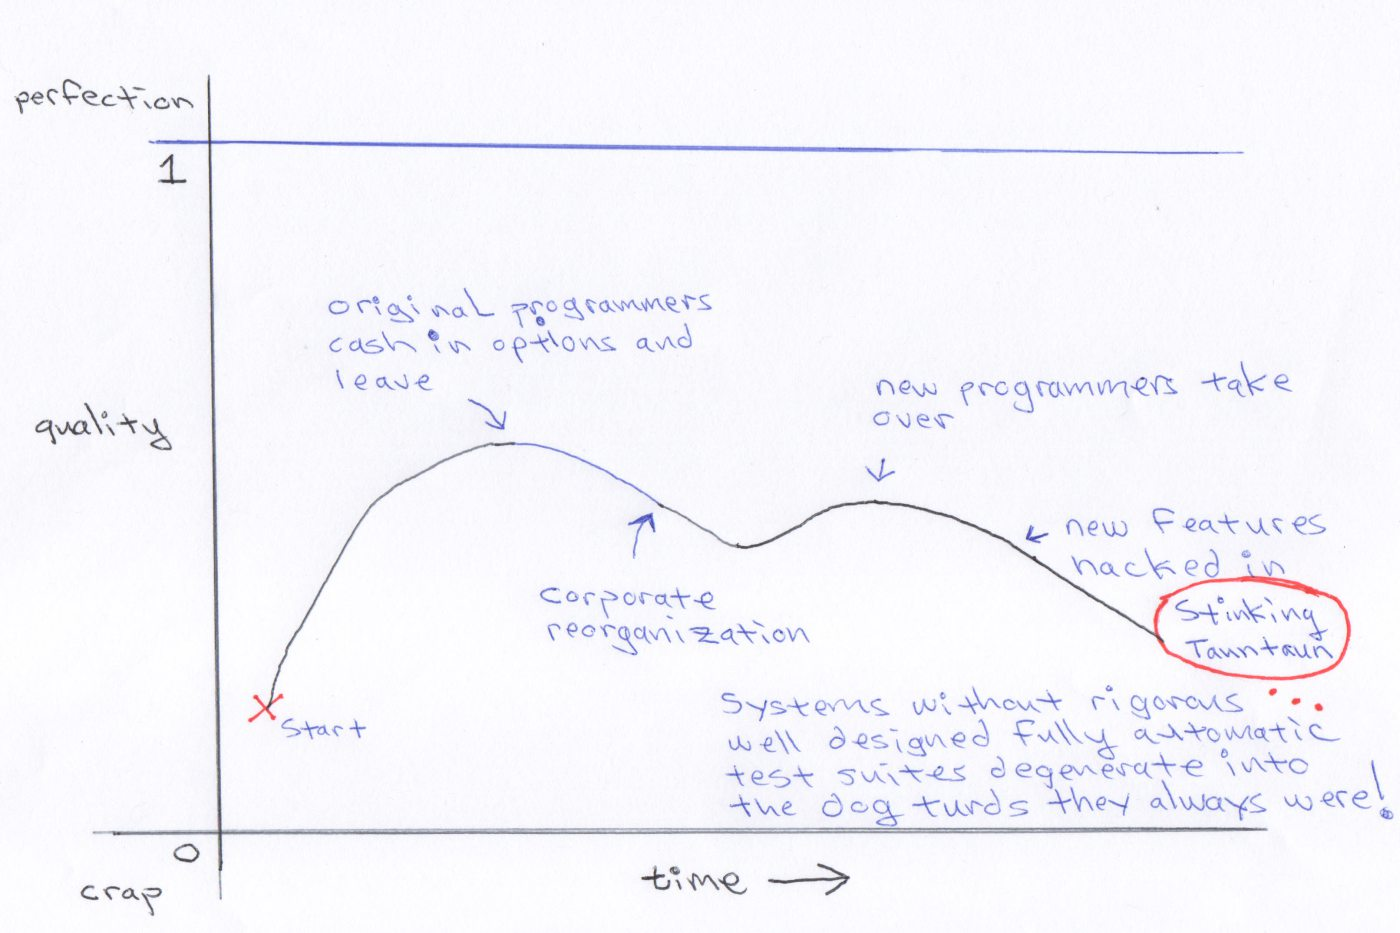
\includegraphics[width=\textwidth]{withouttests.jpg}}
\caption[My \emph{Power-Point-less} illustration of Quality over Time for a system that
lacks a version controlled test suite]{My \emph{Power-Point-less} illustration of Quality over Time for a system that
lacks a \emph{fully automatic ever expanding version controlled test suite.}
Systems without well designed test rigs are almost without exception
complete crap. Unless someone is paying you huge bucks it's best to
start sending out resumes when asked to fix such systems. You can ruin
your health stirring your yummy ice cream into the shit but it's almost
certain the final mixture will taste more like shit than
ice cream.}
\label{fig:4971X1}
\end{figure}



It's the 21\textsuperscript{st} century people! In ENIAC days you could
overlook missing automatic test suites. Nowadays \emph{missing automatic
test suites is a damning indictment of the organization that tolerates
such heinous crimes against programming humanity!}

\medskip
\noindent\textbf{Code Smell \#3: Only one programmer is able to work with legacy
code}.
\medskip

When I was hired there were a few hieroglyphic programmers on staff. No
single programmer was saddled with the accumulated mistakes of prior
decades. We could divide and deal with the pain. During this happy time
our work was support oriented. We we're not undertaking large projects.
Then an inevitable bout of corporate reorganization occurred, followed
by terminations and a stream of defectors fleeing the new order.
Eventually only one hieroglyphic programmer remained\emph{: moi!} Most
programmers would have joined the exodus and not taken on the \emph{sins
of other fathers} but as I have already pointed out I am a software
whore and proud of it. Still even software sluts~must avoid~ending up
like the, ``there can be only one,'' Highlander. Most of those sword
duels \href{https://www.youtube.com/watch?v=_j6_H-PSml0}{ended rather
badly} as I recall.

\medskip
\noindent\textbf{Code Smell \#4: Massive routines with far-ranging name scope.}
\medskip

With noxious fumes already cutting off our air supply we should have
stopped in our tracks but we soldiered on because The Stinking Tauntaun
System did something important and alternatives were not readily
available. The corporation recognized this and started a number of
parallel projects to explore New Stinking Tautaun's. I wasn't lucky
enough to work on any of the parallel projects. I had to get in the
stall and shovel the Tauntaun manure.

We weren't entirely clueless when we started Stinking Tauntaun work.~ We
recognized the precarious hieroglyphic programmer resource constraint
and tried to divide the work into units that alleviated it. We decided
to implement part of the new features in another programming language
and call the new module from the old system. The hope was this would
divide the work and possibly create something that might be used outside
The Stinking Tauntaun System. This part of the project went reasonably
well. The new module is entirely new code and works very well.
Unfortunately, it was~a small part of the greater effort of bolting new
features into The Stinking Tauntaun System.

Stinking Tauntaun code is magisterial in its monolithic madness. The
hieroglyphic programming language is famous for its concise coding style
yet the main routine in the Stinking Tauntaun System is close to 10,000
lines long!~ I had never seen hieroglyphic language routines of such
length. I've only seen comparable programs a few times in my battle
scared career. As a summer student I marveled at a 20,000 line, single
routine, FORTRAN program. At first I thought it was the output of some
cross compiler but no, some insane, bat shit crazy government drone, (I
was working for a government agency in western Canada), had coded it by
hand --- on freaking punch cards no less! Such stunning ineptitude is
rare: most programmers have a passing acquaintance with modular design
and know enough to reconsider things when code gets out of hand. We all
have different thresholds for judging \emph{out-of-hand-ness}, for me
it's any routine that's longer than sixty lines: including the damn
comments.

A 10,000 line routine is a monumental red flag but The Stinking
Tautaun's length was not the biggest problem. There is this thing
programmer's call ``scope.'' Scope marks out name boundaries. It sets
limits on where names have meaning or value. Ideally name scope is
limited to the smallest feasible extent. You really don't want global
names! You absolutely don't want global names like ``\texttt{X},'' or ``\texttt{i},'' or
``\texttt{T},'' cavorting in your code! Most of the cryptic names in the Stinking
Tauntaun System had far-ranging scope. Vast scopes make it difficult to
safely make local changes. This makes it risky, dangerous and
time-consuming to change code. Large scopes also increase the burden on
testers. If tiny changes have far-ranging consequences you have to
retest large parts of the system every time you tweak it. All of this
sucks up time and drains the pure bodily fluids of IT staff.

\medskip
\noindent\textbf{Code Smell \#5: Assumptions about what is possible quickly
prove wrong.}
\medskip


It was looking dark. Timid souls would have run but we plowed on. Our
naive hope rested~on the theory that we could change a few touch points
in The Stinking Tauntaun's code base and then get out of Dodge before
the dark kludge forest closed in. My first estimate of how many routines
I would have to touch was around twenty. Two months into the project I
had already altered over a hundred with no end in sight. The small
orthogonal change we hoped to make was not possible because The Stinking
Tauntaun System did not sensibly do one thing in one place. It did
\emph{sort of the same thing} in many places. You couldn't make a small
change and have things sensibly flow throughout the system. I worked to
isolate and modularize the mess but I should have just waved my hands
and spent my days on LinkedIn looking for another job.

\medskip
\noindent\textbf{Code Smell \#6: A development culture steeped in
SOX inspired counterproductive ceremony.}
\medskip

On top of all these screeching sirens yelling stop there were
other~impediments. I work in a SOX saturated environment. Readers of my
blog know that I consider SOX to be one of the biggest time-wasting
piles of DC idiocies ever pushed on American companies. Like many
``government solutions'' SOX did not drain the intended swamp but
forever saddled us with inane time-wasting ceremony and utterly stupid
levels of micromanagement. Is Active Directory management really a
concern of freaking government? Somehow it's become one!~ One of my
favorite consequences of SOX is the religious ordering of development
environments and the sacraments for promoting code changes. During the
long bruising Stinking Tauntaun project many releases boiled down to me
making changes to one file! Pushing a new version to test should have
been a simple file copy.

Of course it couldn't be that simple. Numerous ``tickets'' had to be
approved. Another branch of IT, that was even more stressed and suffered
higher levels of turnover than ours, was~dragged in to execute a single
trivial file copy. In many cases more bytes were generated by all this
pointless time-wasting ceremony than I had changed in that single file.
Of course all this took time, and as hard as I looked for a
\emph{useless-time-wasting-bullshit} category in our web-based hours
tracking system, I couldn't find one. There's a management mantra: you
can only improve what you measure. Funny how companies never measure
the bullshit.

In retrospect we should have junked The Stinking Tauntaun~System or
opted for a radical rewrite. It's ironic but something like this is
what's going to happen. If I was young I would be bitter but I cashed in
on this project. In my consulting days I was always on the lookout for
Stinking Tauntauns: they were freaking gold mines for those of us that
have acquired a taste for the bracing putrid fumes of rotting code.

% \hyperref[ux5fftnref1]{
% %{[}1{]}
% } If you are the type of person that gets
% your panties in a knot about the \emph{gender of hypothetical supreme
% beings} please go away.

%\captionsetup[floatingfigure]{labelformat=empty}
%\begin{figure}[htbp]
%\begin{floatingfigure}[l]{0.25\textwidth}
%\centering
%\includegraphics[width=0.23\textwidth]{luketauntaun.jpg}
%\caption{~~~IMCAPTION~~~}
%\label{fig:4971X0}
%\end{floatingfigure}
%\end{figure}

%\captionsetup[floatingfigure]{labelformat=empty}
%\begin{figure}[htbp]
%\begin{floatingfigure}[l]{0.25\textwidth}
%\centering
%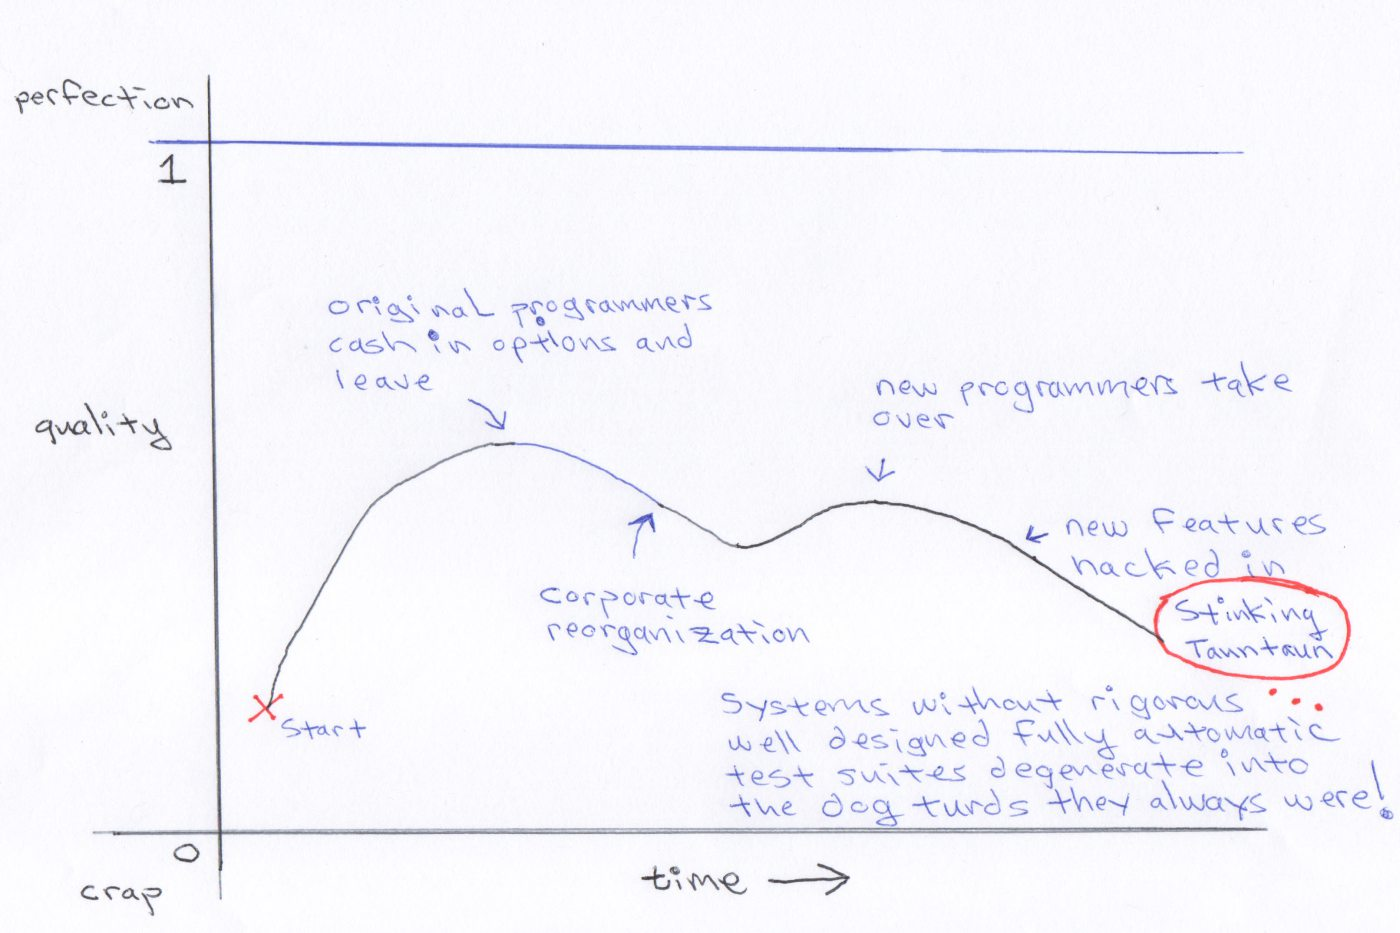
\includegraphics[width=0.23\textwidth]{withouttests.jpg}
%\caption{~~~IMCAPTION~~~}
%\label{fig:4971X1}
%\end{floatingfigure}
%\end{figure}



%\end{document}